\documentclass[notes, 12.5pt, aspectratio=169]{beamer}

\usepackage{pgfpages}
\usepackage{threeparttable}
% These slides also contain speaker notes. You can print just the slides,
% just the notes, or both, depending on the setting below. Comment out the want
% you want.

\setbeameroption{hide notes} % Only slide
%\setbeameroption{show only notes} % Only notes
%\setbeameroption{show notes on second screen=right} % Both


%fonts
%\usepackage{bookman}
%\usepackage[default]{lato}
%\usepackage{helvet}
\usepackage[sc]{mathpazo}
%\usepackage{tex-gyre}


\usepackage{array}
\usepackage{bm}


\usepackage{tikz}
\usepackage{verbatim}
\setbeamertemplate{note page}{\pagecolor{yellow!5}\insertnote}
\usetikzlibrary{positioning}
\usetikzlibrary{snakes}
\usetikzlibrary{calc}
\usetikzlibrary{arrows}
\usetikzlibrary{decorations.markings}
\usetikzlibrary{shapes.misc}
\usetikzlibrary{matrix,shapes,arrows,fit,tikzmark}
\usepackage{amsmath}
\usepackage{mathpazo}
\usepackage{hyperref}
\usepackage{lipsum}
\usepackage{multimedia}
\usepackage{graphicx}
\usepackage{multirow}
\usepackage{graphicx}
\usepackage{dcolumn}
%\usepackage{enumitem}
\usepackage{bbm}
\usepackage[font=small,labelfont=bf]{caption}
\newcolumntype{d}[0]{D{.}{.}{5}}


\usepackage[backend=biber, style=authoryear, citestyle=authoryear, uniquename=false, firstinits=true, maxbibnames=5, minbibnames=1, maxcitenames=2, mincitenames=1, uniquelist=false, datelabel=short, labeldate=year, alldates=year]{biblatex}
\addbibresource{lib_parenting_styles.bib}

\usepackage{changepage}
\usepackage{appendixnumberbeamer}
\newcommand{\beginbackup}{
   \newcounter{framenumbervorappendix}
   \setcounter{framenumbervorappendix}{\value{framenumber}}
   \setbeamertemplate{footline}
   {
     \leavevmode%
     \hline
     box{%
       \begin{beamercolorbox}[wd=\paperwidth,ht=2.25ex,dp=1ex,right]{footlinecolor}%
%         \insertframenumber  \hspace*{2ex} 
       \end{beamercolorbox}}%
     \vskip0pt%
   }
 }
\newcommand{\backupefnd}{
   \addtocounter{framenumbervorappendix}{-\value{framenumber}}
   \addtocounter{framenumber}{\value{framenumbervorappendix}} 
}


\usepackage{graphicx}
\usepackage[space]{grffile}
\usepackage{booktabs}

% These are my colors -- there are many like them, but these ones are mine.
\definecolor{blue}{RGB}{0,114,178}
\definecolor{red}{RGB}{213,94,0}
\definecolor{yellow}{RGB}{240,228,66}
\definecolor{green}{RGB}{0,158,115}

\hypersetup{
  colorlinks=true,
  linkbordercolor = {white},
  linkcolor = {blue}
}


%% I use a beige off white for my background
\definecolor{MyBackground}{RGB}{255,253,218}

%% Uncomment this if you want to change the background color to something else
%\setbeamercolor{background canvas}{bg=MyBackground}

%% Change the bg color to adjust your transition slide background color!
\newenvironment{transitionframe}{
  \setbeamercolor{background canvas}{bg=white}
  \begin{frame}}{
    \end{frame}
}

\setbeamercolor{frametitle}{fg=blue}
\setbeamercolor{title}{fg=black}
\setbeamertemplate{footline}[frame number]
\setbeamertemplate{navigation symbols}{} 
\setbeamertemplate{itemize items}{-}
\setbeamercolor{itemize item}{fg=blue}
\setbeamercolor{itemize subitem}{fg=blue}
\setbeamercolor{enumerate item}{fg=blue}
\setbeamercolor{enumerate subitem}{fg=blue}
\setbeamercolor{button}{bg=MyBackground,fg=blue,}



% If you like road maps, rather than having clutter at the top, have a roadmap show up at the end of each section 
% (and after your introduction)
% Uncomment this is if you want the roadmap!
 \AtBeginSection[]
 {
    \begin{frame}
        \frametitle{Roadmap}
        \tableofcontents[currentsection]
    \end{frame}
 }
\setbeamercolor{section in toc}{fg=blue}
\setbeamercolor{subsection in toc}{fg=red}
\setbeamersize{text margin left=1em,text margin right=1em} 

\newenvironment{wideitemize}{itemize\addtolength{\itemsep}{10pt}}{\enditemize}

\usepackage{environ}
\NewEnviron{videoframe}[1]{
  \begin{frame}
    \vspace{-8pt}
    \begin{columns}[onlytextwidth, T] % align columns
      \begin{column}{.58\textwidth}
        \begin{minipage}[t][\textheight][t]
          {\dimexpr\textwidth}
          \vspace{8pt}
          \hspace{4pt} {\Large \sc \textcolor{blue}{#1}}
          \vspace{8pt}
          
          \BODY
        \end{minipage}
      \end{column}%
      \hfill%
      \begin{column}{.42\textwidth}
        \colorbox{green!20}{\begin{minipage}[t][1.2\textheight][t]
            {\dimexpr\textwidth}
            Face goes here
          \end{minipage}}
      \end{column}%
    \end{columns}
  \end{frame}
}


\makeatletter
\newcommand{\fitimage}[2][\@nil]{
	\begin{figure}
		\begin{adjustbox}{width=0.9\textwidth, totalheight=\textheight-2\baselineskip-2\baselineskip,keepaspectratio}
			\includegraphics{#2}
		\end{adjustbox}
		\def\tmp{#1}%
		\ifx\tmp\@nnil
		\else
		\caption{#1}
		\fi
	\end{figure}
}
\makeatother

\newcommand{\be}{\bm{\beta}}
\newcommand{\x}{\textbf{x}}
\newcommand{\z}{\textbf{z}}
\newcommand{\X}{\textbf{X}}
\newcommand{\Y}{\textbf{Y}}


\title[]{\textcolor{blue}{Measuring Parenting Styles}}
\author[PGP]{}
\institute[ifo]{\small{\begin{tabular}{c c}
\Large Empirical Research on Inequality and Redistribution \\
\large Supervisor: Marc Stöckli \\
\\
\large Florian Schoner   \\
\large ifo  \\
\end{tabular}}}

\date{\today}


\begin{document}

%%% TIKZ STUFF
\tikzset{   
        every picture/.style={remember picture,baseline},
        every node/.style={anchor=base,align=center,outer sep=1.5pt},
        every path/.style={thick},
        }
\newcommand\marktopleft[1]{%
    \tikz[overlay,remember picture] 
        \node (marker-#1-a) at (-.3em,.3em) {};%
}
\newcommand\markbottomright[2]{%
    \tikz[overlay,remember picture] 
        \node (marker-#1-b) at (0em,0em) {};%
}
\tikzstyle{every picture}+=[remember picture] 
\tikzstyle{mybox} =[draw=black, very thick, rectangle, inner sep=10pt, inner ysep=20pt]
\tikzstyle{fancytitle} =[draw=black,fill=red, text=white]
%%%% END TIKZ STUFF

% Title Slide
\begin{frame}
\maketitle
  %\centering The views expressed do not necessarily reflect the position of the Federal Reserve Bank of New York or the Federal Reserve System.
\end{frame}





\section{Motivation}
%\begin{transitionframe}
%  \begin{center}
%    { \Huge \textcolor{black}{Spacing and Words}}
%  \end{center}
%\end{transitionframe}
\begin{frame}{Motivation}
	\begin{columns}
	\begin{column}{1\textwidth}
		\only<1>{\resizebox{0.75\textwidth}{!}{
				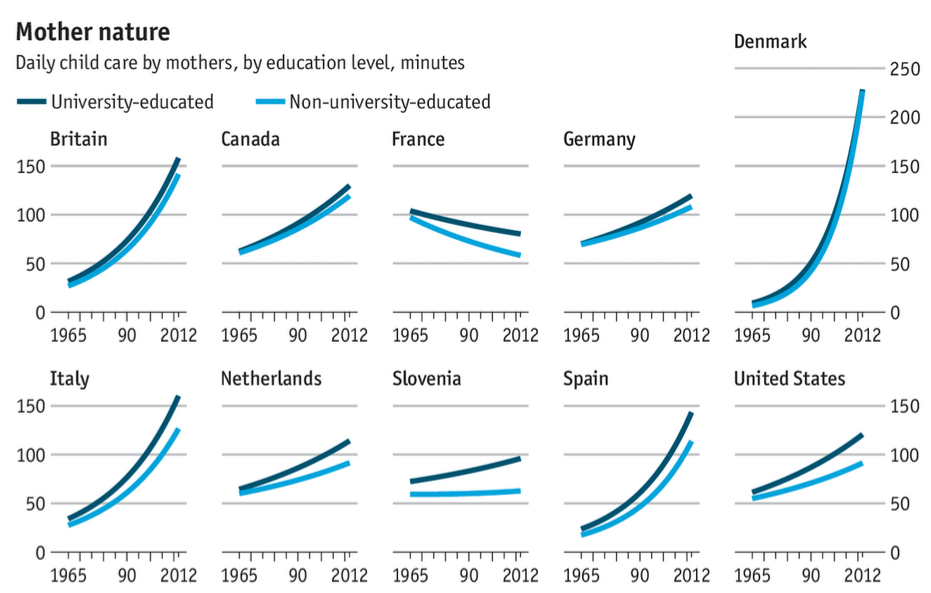
\includegraphics{maternal_time_investments.png}
			}
		\begin{itemize}
			\item[] \footnotesize Source: \url{https://worldinfigures.com/highlights/detail/157}
		\end{itemize}
		}
	\end{column}
	\end{columns}
	\begin{itemize}[(I)]
		\item<2-> Parental (time) investments are an important input to children's technology of skill formation \parencites{falkSocioEconomicStatusInequalities2021}{attanasioEstimatingProductionFunction2020}.
		\vspace{10pt}
		\item<3->  Beyond time investments, parents choose sets of behaviors, ``\textit{parenting styles}'' \parencite{baumrindChildCarePractices1967}, to resolve disagreement about the child's choices (\cite{doepkeParentingStyleAltruism2017, doepkeEconomicsParenting2019}).
		\begin{itemize}
			\item<4-> Authoritative (AV): Parents mold their children's preferences to affect choices.
			\item<5-> Authoritarian (AR): Parents restrict their children's choice set to impose their will.
			\item<6-> Permissive (PE): Parents do not interfere with their children's choices.
		\end{itemize}
		\vspace{10pt}
		\item<7-> Little is known how parenting styles can be measured empirically \parencites{chanParentingStyleYouth2011}{rauhParentingTypes2020}.
		%maybe motivate this with a graph that more educated parents spend more time w/ their children? -> What do they do with their children in that time?! Time trends
	\end{itemize}
\end{frame}
%
\begin{frame}{This paper}
	\begin{itemize}[(I)]
		\item<1-> Research Question: How can we measure parenting styles and its determinants empirically?
		\item[]<2->$\Longrightarrow$ Requires two things:
		\begin{enumerate}
			\item<2-> Data-driven \textbf{classification} of (latent) parenting styles $\rightarrow$ Gaussian Mixture Model \parencite{hastieElementsStatisticalLearning2009}
			\item<3-> Which characteristics \textbf{predict} the choice of parenting styles identified in 1.?
		\end{enumerate}
		\vspace{10pt}
		\item<5-> Data: German National Educational Panel Study \parencite{nepsnationaleducationalpanelstudybamberggermanyNEPSStartingCohort2021}
		\vspace{10pt}
		\item<6-> Results
		\begin{enumerate}
			\item<6-> 3 parenting styles 
			\item<7-> Parental time investment best predicts the choice of a parenting style
		\end{enumerate}
	\end{itemize}
\end{frame}

\section{Data}
\begin{frame}[label=data]{Data: German National Educational Panel Study}
	\begin{itemize}[(I)]
		\item<1-> Panel of 3481 newborns; focus on children's environment and competence development
		\vspace{10pt}
		\item<2-> 3 main types of data
		\begin{enumerate}
			\item<2-> Measures of \textbf{parenting styles} elicit frequency of typical situations between parent and child. $\rightsquigarrow$ Classification exercise
			\item<2-> Measures of \textbf{interaction behaviors} are derived from videotaped recordings of a parent-child play scene $\rightsquigarrow$ Prediction 
			\item<2-> Socio-economic environment $\rightsquigarrow$ Prediction
		\end{enumerate}
	\end{itemize}
\hyperlink{appendix_2}{\beamergotobutton{Descriptives}}
\end{frame}


\section{Classification}
\begin{frame}{Classification: Gaussian Mixture Model}
	\begin{itemize}[(I)]
		\item<1-> Assume that vector of scores of \textbf{parenting styles}, $\bm{x}_i$, $i=1,\ldots,N$ is drawn from a mixture of multivariate normal densities and estimate their parameters
		\item[]<1-> \begin{equation*} f(x) = \sum_{m=1}^{M} \alpha_m \phi(x; \mu_m, \bm{\Sigma}_m) \end{equation*}
		\item<2-> Assign observation to the class (density) where it is most likely to be drawn from \begin{equation*}
			\max_{1 \leqslant m \leqslant M} \widehat{\text{Pr}}(i \in m) = \frac{\widehat{\alpha}_m \phi(x_i; \widehat{\mu}_m, \widehat{\bm{\Sigma}}_m)}{\sum_{k=1}^{M} \widehat{\alpha}_k \phi(x_i; \widehat{\mu}_k, \widehat{\bm{\Sigma}}_k)}
		\end{equation*}
	%\item<3-> Gives assignment probabilities for all classes $\rightsquigarrow$ uncertainty measure
	\end{itemize}
\end{frame}

\section{Results}
\begin{frame}{Results: Classification}
	\makebox[\linewidth][c]{
		\begin{threeparttable}
		\begin{tabular}{lcccccc}
			\hline \hline\\[-1.8ex] 
			&    &    &    &\multicolumn{3}{c}{p-values} \\ 
			\cline{5-7} \\[-1.8ex]Dimension & 1 & 2 & 3 & 1/2 & 1/3 & 2/3 \\ 
			\midrule
			Powerful enforcement & \marktopleft{a1}0.033 & 0.057 & $-$0.066 \markbottomright{a1}{red} & 0.596 & 0.001 & 0.004 \\ 
			%Emotional warmth & 0.130 & 0.370 & $-$0.241 & 0.000 & 0.000 & 0.000 \\ 
			%Inconsistent parent. & $-$0.101 & $-$0.095 & 0.112 & 0.641 & 0.000 & 0.000 \\ 
			%Neg. communication & $-$0.076 & $-$0.235 & 0.177 & 0.000 & 0.000 & 0.000 \\ 
			Monitoring & \marktopleft{a2} 0.099 & 0.290 & $-$0.199 \markbottomright{a2}{red}& 0.000 & 0.000 & 0.000 \\ 
			Autonomy & \marktopleft{a3}$-$0.007 & 0.191 & $-$0.066 \markbottomright{a3}{red}& 0.000 & 0.000 & 0.000 \\ 
			%Pos. parent. behavior & $-$0.097 & 0.669 & $-$0.136 & 0.000 & 0.485 & 0.000 \\ 
			%Psychological control & $-$0.127 & $-$0.100 & 0.137 & 0.178 & 0.000 & 0.000 \\ 
			\hline \bottomrule
		\end{tabular}
	\begin{tablenotes}
		\small
		\item \textit{Notes}: Class means of the different parenting styles dimensions based on $N = 1504$ observations. P-values for $t$-tests on equality of means against a two-sided alternative.
	\end{tablenotes}
	\end{threeparttable}
	}
\uncover<1-1>{\tikz[overlay,remember picture,inner sep=1pt]
	\node[draw=red,rounded corners,fit=(marker-a1-a.north west) (marker-a1-b.south east)] {};}
\uncover<2-2>{\tikz[overlay,remember picture,inner sep=1pt]
	\node[draw=red,rounded corners,fit=(marker-a2-a.north west) (marker-a2-b.south east)] {};}
\uncover<3-3>{\tikz[overlay,remember picture,inner sep=1pt]
	\node[draw=red,rounded corners,fit=(marker-a3-a.north west) (marker-a3-b.south east)] {};}
\end{frame}

\begin{frame}{Results: Multinomial Logit (i)}
	\begin{itemize}[(I)]
		\item<1-> Do differences in parent-child interaction behavior and/or socio-economics characteristics predict the choice of parenting style?
		\item[]<2-> \begin{equation*} \text{Pr}(\text{parenting style}_i = m) = \frac{\exp(\x^\top_{i} \be_m + \z^\top_{i} \bm{\gamma}_m)}{\sum_{l=1}^{3} \exp(\x^\top_{i}\be_l + \z^\top_{i} \bm{\gamma}_l)},  \label{eq:multinom}
		\end{equation*}
		\begin{itemize}
			\item <2-> $m$: either authoritative, authoritarian, or permissive
			\item <2-> $\x_i$ contains measures of parental interaction behavior
			\item <2-> $\z_i$ captures the child's socio-economic environment
		\end{itemize} 
	\end{itemize}
\end{frame}

\begin{frame}[label=main_results]{Results: Multinomial Logit (ii)}
	\setbeamercovered{invisible}
	\makebox[\linewidth][c]{
	\footnotesize
	%\begin{threeparttable}
		\begin{tabular}[t]{<{\onslide<1->}ll c<{\onslide<2->}c<{\onslide}}
			\hline \hline \\[-1.8ex]
			%&    &  \multicolumn{2}{c}{Multinomial Logit}\\
			%&    &  \multicolumn{2}{c}{Dep. var.: Parenting style}\\
			&    & (1) & (2) \\
			\cline{3-4} \\[-1.8ex]
			Sensitivity & AR & 0.731** (0.158) & 0.762 (0.165)\\
			& AV & 0.833 (0.117) & 0.812* (0.121)\\
			&  &  \vphantom{4} & \\
			Intrusiveness & AR & 0.812 (0.138) & 0.791 (0.144)\\
			& AV & 0.817** (0.103) & 0.809** (0.106)\\
			&  &  \vphantom{3} & \\
			Detachment & AR & 0.896 (0.107) & 0.920 (0.109)\\
			& AV & 0.944 (0.075) & 0.940 (0.076)\\
			&  &  \vphantom{2} & \\
			Emotionality & AR & 1.397** (0.161) & 1.477** (0.168)\\
			& AV & 1.036 (0.120) & 1.046 (0.123)\\
			&  &  \vphantom{1} & \\
			%Siblings & AR &  & 1.146 (0.207)\\
			%& AV &  & 1.057 (0.152)\\
			%&  &  & \\
			Time investment & AR &  & 2.332*** (0.112)\\
			& AV &  & 1.516*** (0.078)\\
			\midrule
			Further controls &  & No & Yes\\
			N &  & 1002 & 1002\\
			\bottomrule
		\end{tabular}
%		\begin{tablenotes}
%			\small
%			\item \textit{Notes}: Multinomial logit estimates. Parental interaction behaviors include Sensitivity, Intrusiveness, Detachment, Stimulation,
%			Positive Regard, Negative Regard, and Emotionality. Further controls include Mother's age, High school, Income, High-SES, Siblings,
%			Married, Migration background.
%			***, **, * indicate significance at the 1\%, 5\%, and 10\% level,
%			respectively.
%		\end{tablenotes}
%	\end{threeparttable}
}
\hyperlink{appendix_1}{\beamergotobutton{Full table}}
\end{frame}

\section{Conclusion}
\begin{frame}{Conclusion}
	\begin{itemize}
		\item<1-> Use unsupervised ML to classify parenting styles which are partly in line with \textcite{baumrindChildCarePractices1967}
		\vspace{10pt}
		\item<2-> The classification's results are best predicted by differences in parental time investment $\rightarrow$ family structure important
		\vspace{10pt}
		\item[]<3-> Outlook:
		\begin{enumerate}
			\item Time investment: Only look at children without siblings?
			\item Use parental interaction behaviors for classification?
			\item Investigate children's test scores.
		\end{enumerate}
	\end{itemize}
\end{frame}

\begin{frame}%%     1
	\begin{center}
		\Huge Thank You!
	\end{center}
\end{frame}


\begin{frame}[allowframebreaks]
	\printbibliography
\end{frame}

\section{Appendix}

\appendix

\begin{frame}[label=appendix_1]{}
	\setbeamercovered{invisible}
	\makebox[\linewidth][c]{
		\tiny
		\begin{tabular}[t]{llccc}
			\hline \hline \\[-1.8ex]
			%&    &  \multicolumn{2}{c}{Multinomial Logit}\\
			%&    &  \multicolumn{2}{c}{Dep. var.: Parenting style}\\
			\hyperlink{main_results}{\beamergotobutton{Back}}&    & (1) & (2) \\
			\cline{3-4} \\[-1.8ex]
			%(Intercept) & AR & 0.408*** (0.095) & 0.643 (0.312)\\
			%& AV & 1.142* (0.070) & 1.218 (0.240)\\
			
			Sensitivity & AR & 0.731** (0.158) & 0.762 (0.165)\\
			& AV & 0.833 (0.117) & 0.812* (0.121)\\
			
			Intrusiveness & AR & 0.812 (0.138) & 0.791 (0.144)\\
			& AV & 0.817** (0.103) & 0.809** (0.106)\\
			
			Detachment & AR & 0.896 (0.107) & 0.920 (0.109)\\
			& AV & 0.944 (0.075) & 0.940 (0.076)\\
			
			Stimulation & AR & 1.103 (0.126) & 0.942 (0.132)\\
			& AV & 1.145 (0.093) & 1.046 (0.098)\\
			
			Pos. Regard & AR & 0.939 (0.149) & 0.966 (0.155)\\
			& AV & 1.107 (0.109) & 1.142 (0.112)\\
			
			Neg. Regard & AR & 0.940 (0.100) & 0.934 (0.104)\\
			& AV & 0.973 (0.074) & 0.978 (0.076)\\
			
			Emotionality & AR & 1.397** (0.161) & 1.477** (0.168)\\
			& AV & 1.036 (0.120) & 1.046 (0.123)\\
			`Mother's age` & AR &  & 0.863 (0.107)\\
			& AV &  & 0.948 (0.078)\\
			
			`High school` & AR &  & 0.639* (0.234)\\
			& AV &  & 0.927 (0.175)\\
			
			Income & AR &  & 1.112 (0.096)\\
			& AV &  & 1.068 (0.073)\\
			
			`High-SES` & AR &  & 0.616* (0.260)\\
			& AV &  & 0.878 (0.195)\\
			
			Siblings & AR &  & 1.146 (0.207)\\
			& AV &  & 1.057 (0.152)\\
			
			Time investment & AR &  & 2.332*** (0.112)\\
			& AV &  & 1.516*** (0.078)\\
			
			Married & AR &  & 0.942 (0.274)\\
			& AV &  & 1.145 (0.206)\\
			`Migration background` & AR &  & 1.331 (0.218)\\
			& AV &  & 0.941 (0.166)\\
			\midrule
			N &  & 1002 & 1002\\
			\bottomrule
		\end{tabular}
	}
	\hyperlink{main_results}{\beamergotobutton{Back}}
\end{frame}

\begin{frame}[label=appendix_2]{}
	\makebox[\linewidth][c]{
		\footnotesize
	\begin{table}[!htbp]
		\centering
		\begin{threeparttable}
			%\caption{Summary Statistics}
			\label{tab:summ_stats}
			\begin{tabular}[t]{lcccccc}
				\hline\hline\\[-1.8ex] 
				\multicolumn{1}{c}{ \hyperlink{data}{\beamergotobutton{Back}}} & \multicolumn{2}{c}{High (N=1032)} & \multicolumn{2}{c}{Low (N=395)} & \multicolumn{1}{c}{    } & \multicolumn{1}{c}{    } \\
				\cmidrule(l{3pt}r{3pt}){2-3} \cmidrule(l{3pt}r{3pt}){4-5}
				& Mean & Std. Dev. & Mean  & Std. Dev.  & Mean Diff. & p-val.\\
				\midrule
				A. Child characteristics &&&&&&           \\
				\hspace{5mm}Female & 0.495 & 0.500 & 0.491 & 0.501 & -0.004 & 0.892\\
				\hspace{5mm}Migration back. & 0.316 & 0.463 & 0.462 & 0.499 & 0.146 & 0.000\\
				\hspace{5mm}Siblings & 0.736 & 0.871 & 0.653 & 0.903 & -0.083 & 0.116\\
				B. Family characteristics &&&&&&           \\
				\hspace{5mm}Married & 0.803 & 0.349 & 0.705 & 0.404 & -0.099 & 0.000\\
				\hspace{5mm}High School & 0.784 & 0.412 & 0.333 & 0.472 & -0.450 & 0.000\\
				\hspace{5mm}Unemployed & 0.199 & 0.398 & 0.233 & 0.423 & 0.034 & 0.174\\
				\hspace{5mm}Mother's age & 33.663 & 4.271 & 31.312 & 5.022 & -2.350 & 0.000\\
				\hspace{5mm}Income & 4496.568 & 2274.691 & 3308.075 & 1294.929 & -1188.494 & 0.000\\
				\hspace{5mm}Time investment* & 0.080 & 0.978 & -0.236 & 1.037 & -0.316 & 0.000\\
				C. Interaction behaviors &&&&&&           \\
				\hspace{5mm}Sensitivity* & 0.108 & 0.939 & -0.316 & 1.076 & -0.424 & 0.000\\
				\hspace{5mm}Intrusiveness* & -0.074 & 0.937 & 0.257 & 1.143 & 0.331 & 0.000\\
				\hspace{5mm}Detachment* & -0.023 & 0.949 & 0.069 & 1.114 & 0.092 & 0.185\\
				\hspace{5mm}Stimulation* & 0.072 & 0.967 & -0.185 & 1.058 & -0.258 & 0.000\\
				%\hspace{5mm}Pos. Regard* & 0.082 & 0.967 & -0.212 & 1.043 & -0.294 & 0.000\\
				%\hspace{5mm}Neg. Regard* & -0.048 & 0.927 & 0.179 & 1.212 & 0.227 & 0.002\\
				\hspace{5mm}Emotionality* & 0.098 & 0.961 & -0.194 & 1.044 & -0.292 & 0.000\\
				\hline\hline
			\end{tabular}
			\begin{tablenotes}
				\tiny
				\item \textit{Notes}: Summary statistics of $N = 1427$ observations stratified by SES. P-values are for $t$-tests on equality of means against a two-sided alternative. Female is a dummy indicating whether a child's sex is female. Migration background indicates whether the child has any migration background. Siblings is a dummy indicating whether there are siblings born prior to the surveyed child's birth. Married is a dummy indicating whether the respondent is married. Unemployed is a dummy indicating whether the respondent was unemployed one year prior to child birth. Time investment is generated as the sum of a range of items capturing the frequency of highly-interactive parent-child activities.\\ *: Variable has been standardized to have mean zero and standard deviation equal to one.
			\end{tablenotes}
		\end{threeparttable}
	\end{table}
}
\end{frame}
%
%\begin{frame}[label=appendix_end]{Use it to intimidate audiences!}
%  \begin{itemize}
%    \item[] Now you can make it clear you've done a shitload of work
%      \begin{itemize}
%      \item[]  without having to show everything! \hyperlink{appendix_start}{\beamergotobutton{Back}}
%      \end{itemize}
%    \item[] You label a frame with the \texttt{[label=name]} option, and then point a link to it
%    \item[] You can make an object a link using the \texttt{\textbackslash hyperlink\{label\}\{object\}} command
%  \end{itemize}
%\end{frame}



\end{document}
